%-----------------------------------------------------------------------------
%
%               Template for sigplanconf LaTeX Class
%
% Name:         sigplanconf-template.tex
%
% Purpose:      A template for sigplanconf.cls, which is a LaTeX 2e class
%               file for SIGPLAN conference proceedings.
%
% Guide:        Refer to "Author's Guide to the ACM SIGPLAN Class,"
%               sigplanconf-guide.pdf
%
% Author:       Paul C. Anagnostopoulos
%               Windfall Software
%               978 371-2316
%               paul@windfall.com
%
% Created:      15 February 2005
%
%-----------------------------------------------------------------------------


\documentclass[preprint]{sigplanconf}

% The following \documentclass options may be useful:

% preprint      Remove this option only once the paper is in final form.
% 10pt          To set in 10-point type instead of 9-point.
% 11pt          To set in 11-point type instead of 9-point.
% numbers       To obtain numeric citation style instead of author/year.

\usepackage{amsmath}
\usepackage[pdftex]{graphicx}
\usepackage{float}
\graphicspath{{images/}}

\newcommand{\cL}{{\cal L}}

\begin{document}

\special{papersize=8.5in,11in}
\setlength{\pdfpageheight}{\paperheight}
\setlength{\pdfpagewidth}{\paperwidth}

\conferenceinfo{CONF 'yy}{Month d--d, 20yy, City, ST, Country}
\copyrightyear{20yy}
\copyrightdata{978-1-nnnn-nnnn-n/yy/mm}
\copyrightdoi{nnnnnnn.nnnnnnn}

% Uncomment the publication rights you want to use.
%\publicationrights{transferred}
%\publicationrights{licensed}     % this is the default
%\publicationrights{author-pays}

\titlebanner{banner above paper title}        % These are ignored unless
\preprintfooter{short description of paper}   % 'preprint' option specified.

\title{High-Performance Persistent Graphs}
\subtitle{}

\authorinfo{John Moody}
           {Colorado College '16}
           {john.moody@coloradocollege.edu}
\authorinfo{Benjamin Ylvisaker}
           {Assistant Professor, Colorado College}
           {ben.ylvisaker@coloradocollege.edu}

\maketitle

%should there be some kind of general comment about the current state of persistent data structures, either here or in the introduction?

\begin{abstract}
In the world of persistent data structures, there exist few high performance graph libraries.
We propose in this paper a C library which stores an application-controlled persistent graph in a structure derived from a hash array mapped trie, using chunking and lazy copying to conserve memory and increase performance.
We achieve -some stuff about time complexity that I haven't figured out yet-.
\end{abstract}

\category{CR-number}{subcategory}{third-level}

\keywords
persistent data structures, graphs, hash array mapped trie

\section{Introduction}

A graph is defined as a structure containing some number of nodes and some number of edges, which connect nodes together.
The graph is a data structure with wide-ranging applications, from computational graphs to databases, networking and pathfinding.
To get information about nodes or edges in a graph within a program we typically use an array or some manner of key-value store.
The value associated with a node is usually a list of adjacent nodes, which are either predecessors to that node or antecedents.
We will explore what it means for a graph to be stored in a persistent way, and then propose a structure with strong performance characteristics for various operations and optimized use of memory.

\subsection{Persistence}
What does it mean for data to be stored in a persistent way?
A piece of data is persistent if it does not change.
Consider a linked list in memory, Jeff:
\begin{figure}[H]
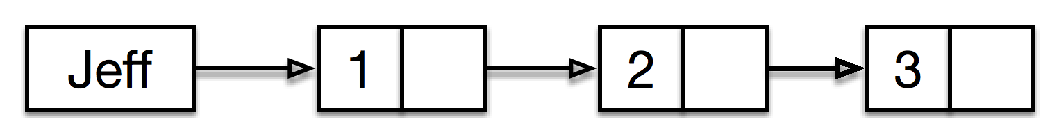
\includegraphics[scale=.35]{linkedlist}
\centering
\end{figure}
There are a number of ways to make an edit to this structure.
If we wanted to change the frontal value of Jeff from 1 to 5, and we do not need the original any longer, we may simply change it:
\begin{figure}[H]
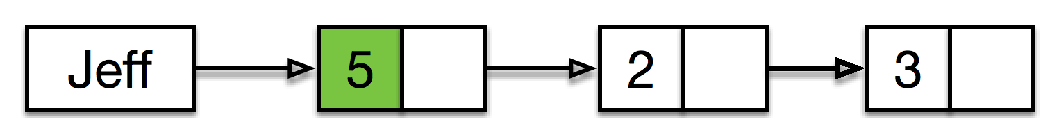
\includegraphics[scale=.35]{linkedlist2}
\centering
\end{figure}
If we want this notion of persistence to apply to Jeff, however, Jeff cannot change.
Instead, we need to come up with a way to change the front value of Jeff to 5 while keeping the original version of Jeff with 1 at the front intact.
Enter "Jeff'":
\begin{figure}[H]
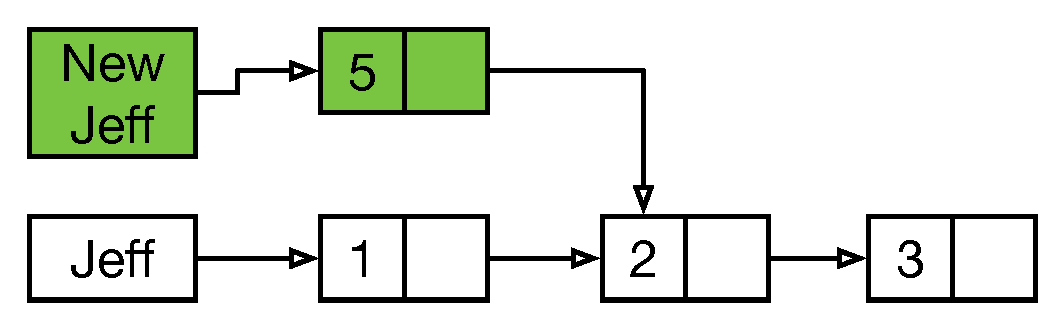
\includegraphics[scale=.35]{linkedlist3}
\centering
\end{figure}
Jeff, we notice, has not changed.
Jeff' preserves the parts of Jeff's structure that they have in common.
Persistent data structures, then, refer to structures like Jeff and Jeff', which, after being created, will always remain the same.

\subsubsection{Trees and Reference Counting}
Let us now consider an example using a simple binary search tree, where we have D, and a separate copy D':
\begin{figure}[H]
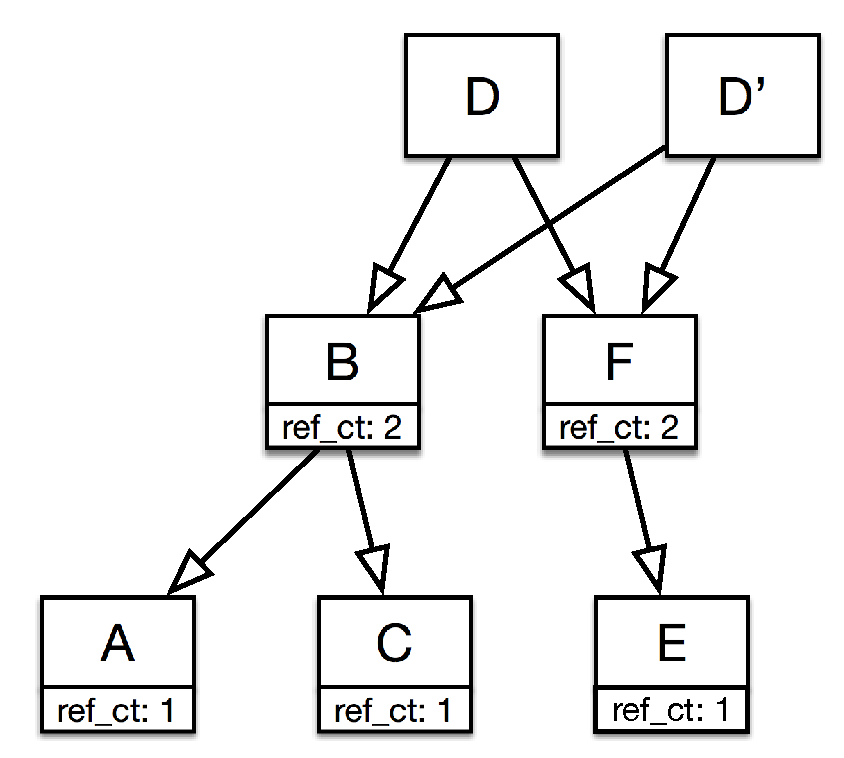
\includegraphics[scale=.43]{treefig}
\centering
\end{figure}
For us to be able to make edits to D' without changing D, we must introduce the concept of reference counting.
A reference count keeps track of how many objects point to a given node.
Here, since B and F have reference counts greater than one, we know that we can't modify those nodes without changing another version of the data structure.
Therefore, when we insert G into D', we will copy any nodes that have reference counts greater than one and adjust the tree as necessary:
\begin{figure}[H]
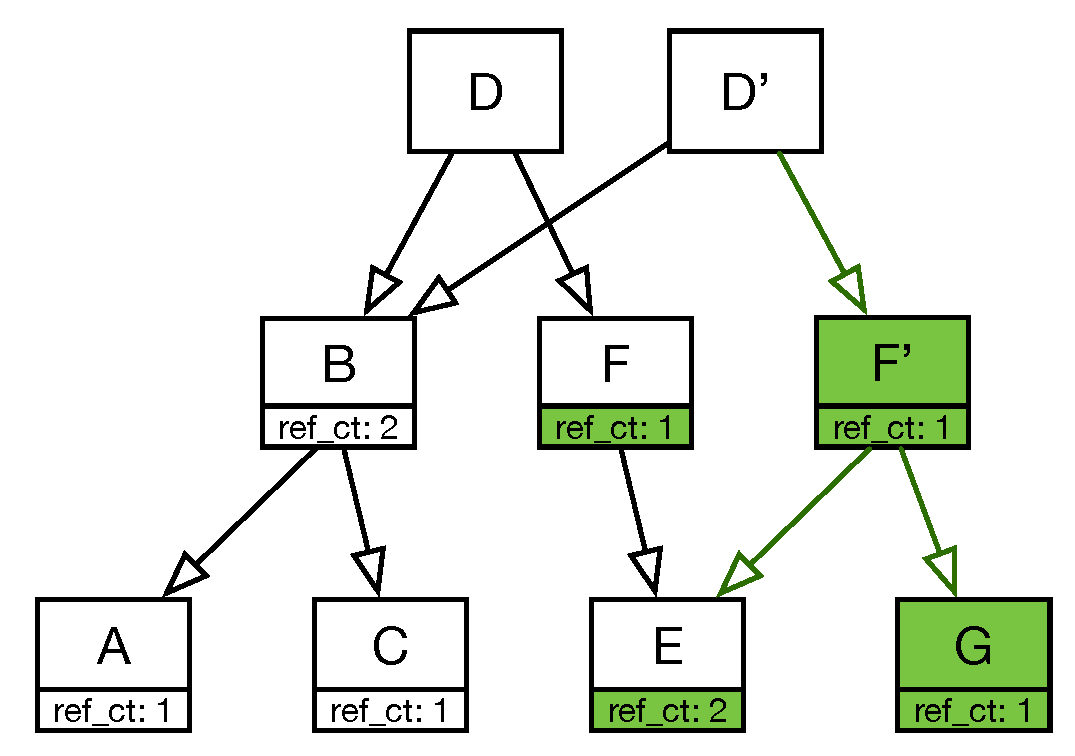
\includegraphics[scale=.43]{treefig2}
\centering
\end{figure}
\subsection{Tries}
How do we represent a graph persistently? We know that whatever structure we use, if we want to efficiently store memory between versions, needs to have elements of tree-like structure, with pointers between them.
A simple binary search tree is possible, and is used for some persistent graph libraries.
However, the use of a binary search tree introduces significant memory inefficiency.






\appendix
\section{Appendix Title}

This is the text of the appendix, if you need one.

\acks

Acknowledgments, if needed.

% We recommend abbrvnat bibliography style.

\bibliographystyle{abbrvnat}

% The bibliography should be embedded for final submission.

\begin{thebibliography}{}
\softraggedright

\bibitem[Smith et~al.(2009)Smith, Jones]{smith02}
P. Q. Smith, and X. Y. Jones. ...reference text...

\end{thebibliography}


\end{document}
